\documentclass[reprint,english,notitlepage]{revtex4-2}
\usepackage{amsmath}
\usepackage[mathletters]{ucs}
\usepackage[utf8x]{inputenc}
\usepackage[english]{babel}
\usepackage{esint}
\usepackage{physics,amssymb}
\usepackage{graphicx}
\usepackage{xcolor}
\usepackage{hyperref}
\usepackage{listings}
\usepackage{subfigure}
% \usepackage[style=science, backend=biber]{biblatex}
% \addbibresource{Report_Part_5.bib} TODO: Slett før innlevering
\hypersetup{
    colorlinks,
    linkcolor={red!50!black},
    citecolor={blue!50!black},
    urlcolor={blue!80!black}}

\lstset{inputpath=,
    backgroundcolor=\color{white!88!black},
    basicstyle={\ttfamily\scriptsize},
    commentstyle=\color{magenta},
    language=Python,
    morekeywords={True,False},
    tabsize=4,
    stringstyle=\color{green!55!black},
    frame=single,
    keywordstyle=\color{blue},
    showstringspaces=false,
    columns=fullflexible,
    keepspaces=true}

\begin{document}

\title{Interplanetary Rocket Launch}
\author{Candidates: 15369 \& 15401}
\date{\today}
\affiliation{Institute of Theoretical Astrophysics, University of Oslo}

\begin{abstract}
    The spacecraft was launched on the 19th July of the year 238 from planet 0 at an angle of $260.483^{\circ}$ and successfully reached space after 16 minutes and 36 seconds.
    It entered the predetermined trajectory at an angle of to planet 1 and followed it using multiple correctional boosts until reaching its destination.
    After reaching planet 1, the spacecraft slowed as part of an orbital injection maneuver to enter a circular orbit at an altitude of 75'000 km above the surface.
    By calculating the orbit as a two body system right after the injection maneuver and after multiple orbits of the spacecraft around the planet, we were able to confirm that the orbit was circular and stable.
\end{abstract}
\maketitle

\section{Introduction} \label{sec:introduction}
The purpose of this project is the launch of our shuttle.
Interplanetary travel have huge cost and risks.
Therefore, we must guarantee success by planning ahead of our journey.
We will develop a simulation to visualize our orbit given some parameters as a means to get a good picture of where we will end up.\\

After completing these final preparations and simulations, we will then send our spacecraft towards its destination.
The launch and interplanetary travel will be executed based on the calculations and simulations we have done in the previous parts of this series of reports.
However, as we have done some assumptions and simplifications in our simulations, we expect some deviations in the actual path of the spacecraft.
This is due to factors such as solar winds, gravitational forces from small objects and friction.\\
To reach our destination, we will therefore launch the rocket on the simulated trajectory and do some corrections of our trajectory, if the actual trajectory deviates from the simulated trajectory.\\
These corrections will be done by firing our rocket engine to change our velocity, and therefore our trajectory as described in figure~\ref{fig:boost_fig}.

\begin{figure}[h]
    %% H(Here), h(here approx), t(top of page), b(bottom of page)
    \centering
    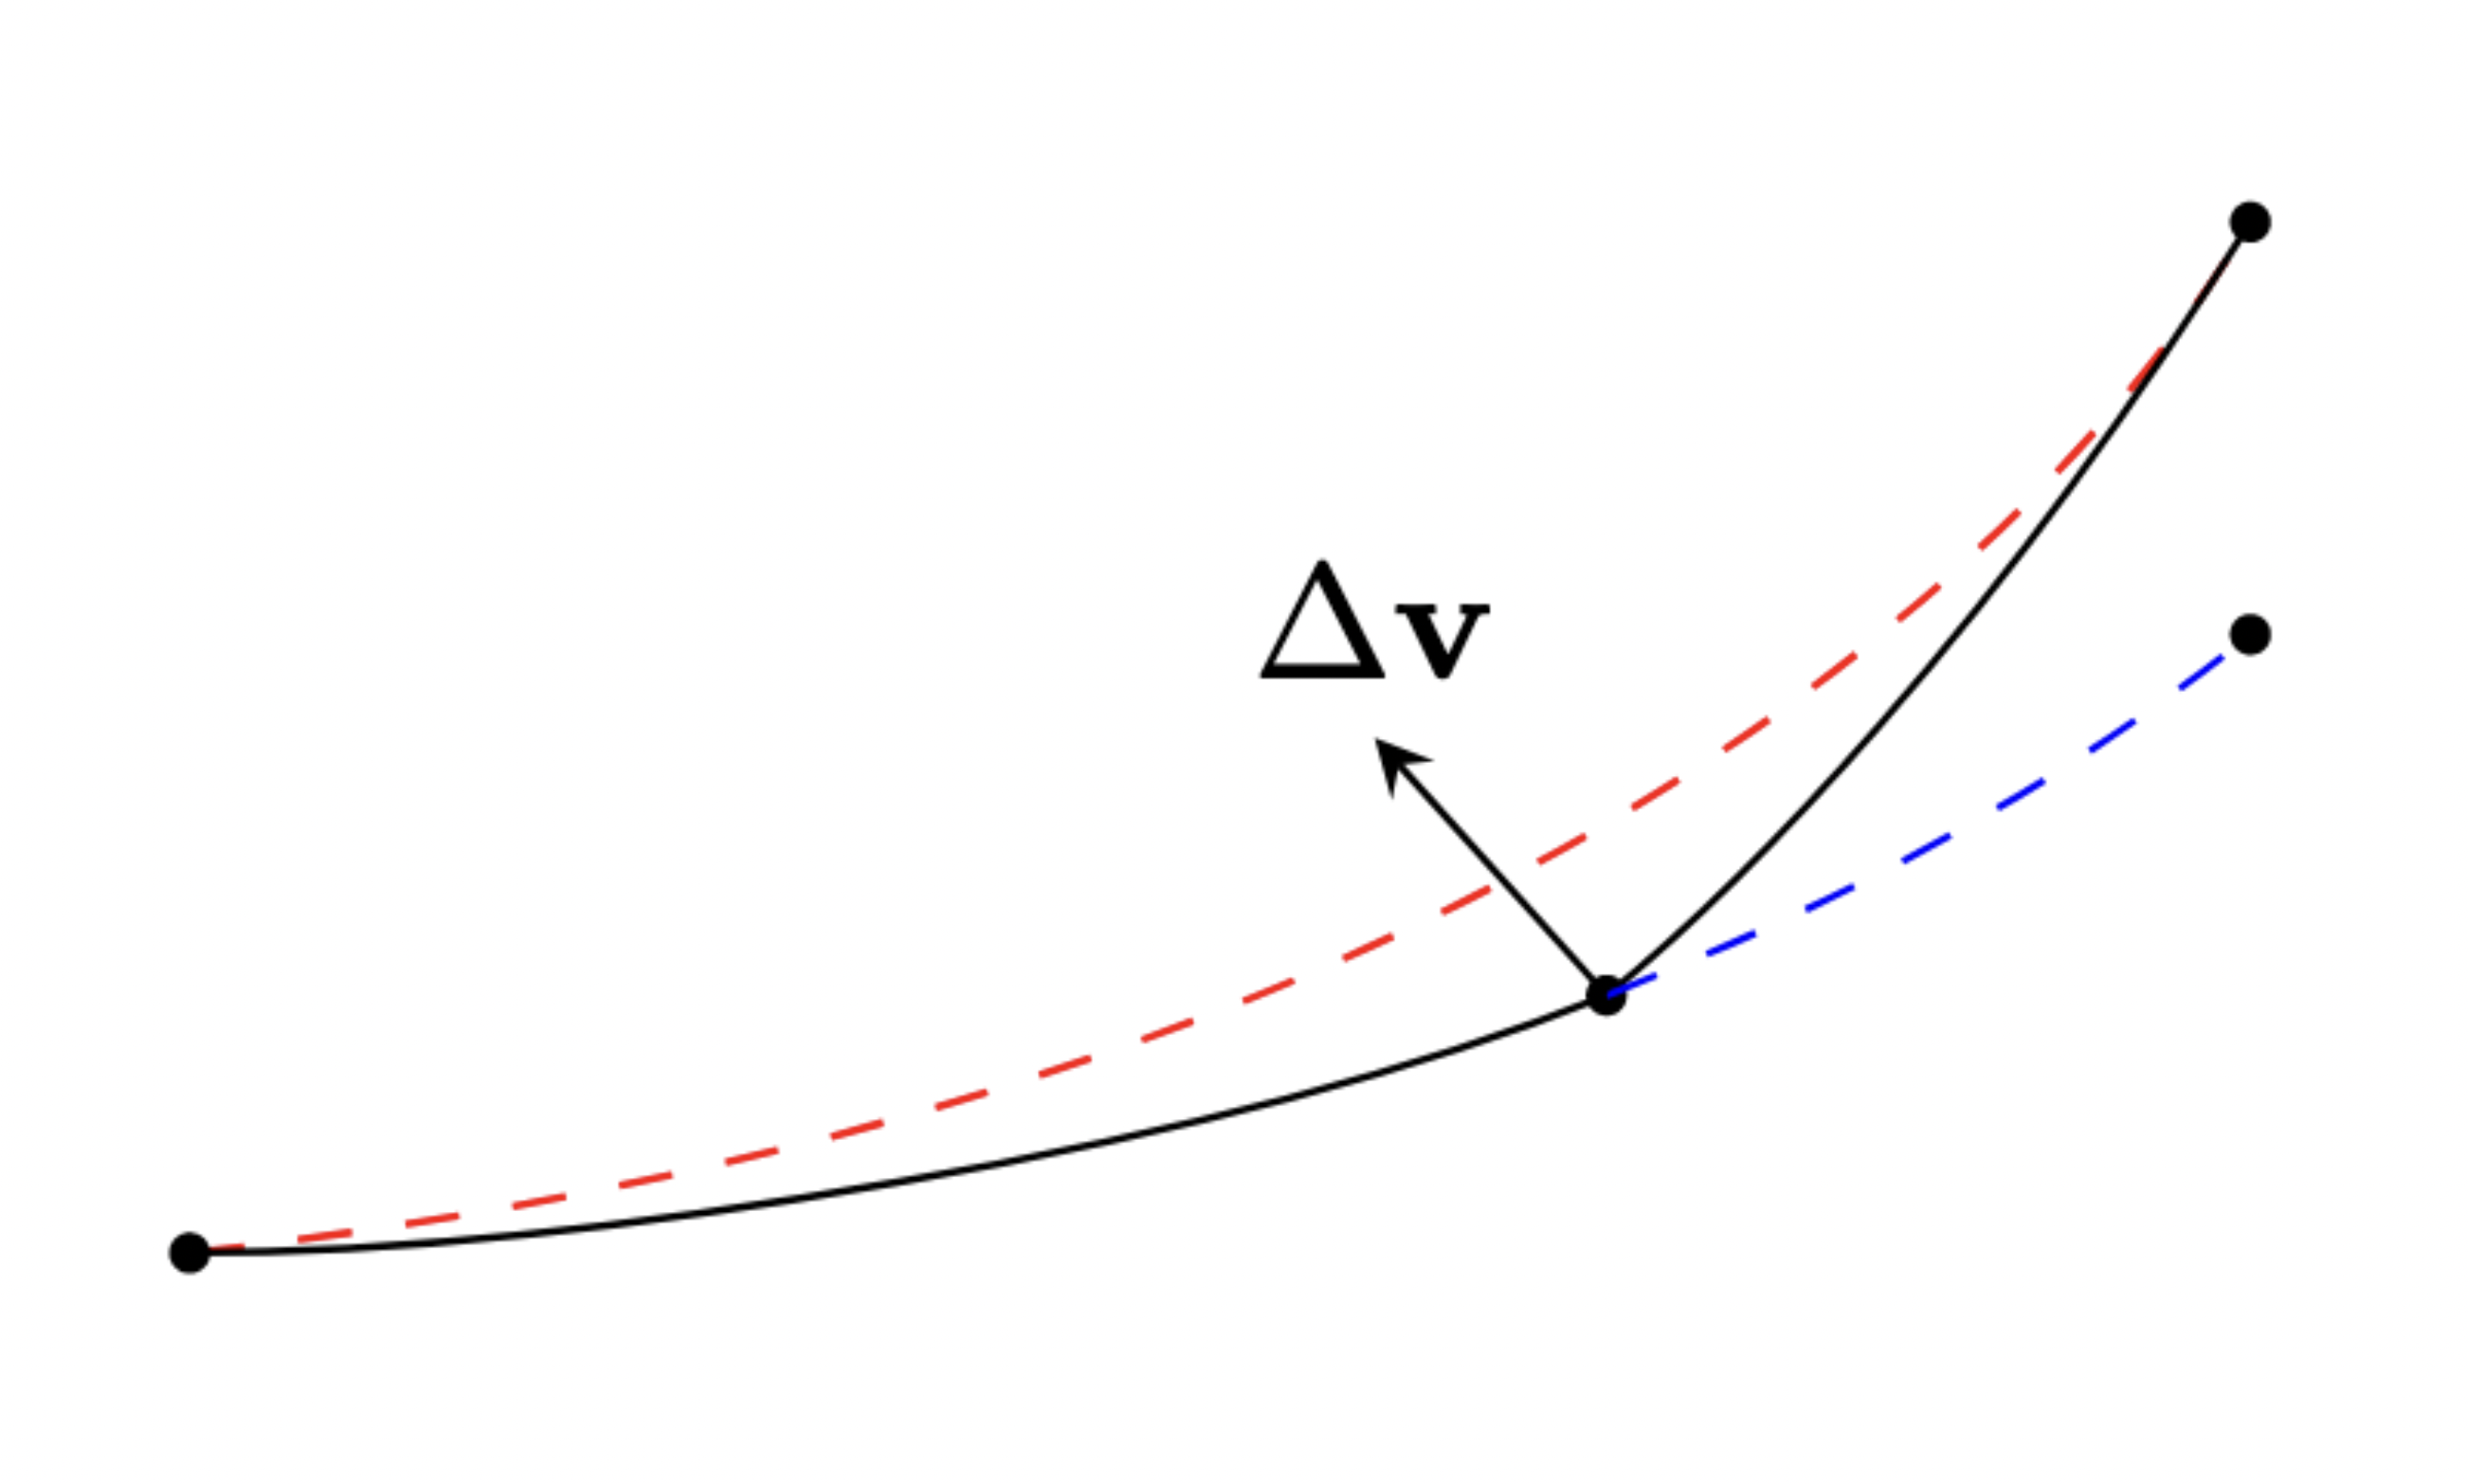
\includegraphics[scale=0.12]{Figures/boost_fig}
    \caption{Visualisation of a correctional boost to change the trajectory. The actual trajectory (black) deviates from the planned trajectory (red), then a trajectory
        correction $\Delta v$ is used to prevent the trajectory from drifting further away (blue). From %~\parencite[][]{project_description5} TODO: Remove Comment
    }\label{fig:boost_fig}
\end{figure}

The goal is to get close enough to the planet so that the gravitational forces from the planet dominate over the gravitational forces from the rest of the planets and the star.
We can then initialise an orbit injection maneuver to enter the orbit around the planet.\\

When in orbit around the destination planet, we will have to orient ourselves and analyze the orbit we are in.
Using the onboard instruments we will determine all necessary parameters to be able to fully simulate the orbit.
This is to predict the movement and position of our spacecraft at a later point in time, which will be necessary to determine a time and position for the landing of our rover.
Furthermore, we can determine the stability of the orbit based on its shape.
The more eccentric an orbit is, the more unstable it is.



\section{Theory} \label{sec: theory}
A description of the Leapfrog simulation method can be found in section II of the second paper %~\parencite[][]{part2} TODO: Delete Comment.
of this series of papers


\section{Method} \label{sec: method}
\subsection{Simulating trajectory} \label{ssec: simulating trajectory}
To simulate the trajectory our shuttle we will calculate all the forces acting upon it.
Using Newton's second law of motion we get this expression for the acceleration the shuttle will experience on its journey.
\[
\mathbf{a} = - G \frac{M_{\text{star}}}{\mathbf{\left\vert \mathbf{r} \right\vert ^{3}}} \mathbf{r} - \sum_{i} G \frac{m_i}{\left\vert \mathbf{r} - \mathbf{r}_i \right\vert ^{3}} \left( \mathbf{r} - \mathbf{r}_i \right)
\]
Starting from the left, $ \mathbf{a} $ is the acceleration of the shuttle, $ G $ the gravitational constant, $ M_{\text{star}} $ the mass of the star and $ \mathbf{r} $ is the position of the shuttle.
We then add the sum of the acceleration from the planets in the solar system where $ m_i $ and $ \mathbf{r}_i $ is the mass and position of each planet respectively.
The shuttle has an insignificant amount of mass, and we will ignore it during our calculations.

Then we use the Leapfrog integration method get the next position after a small amount of time $ \Delta t $ has passed as shown in the equations below

\begin{subequations} \label{eq: leapfrog integration}
    \begin{equation}
        v_{i + \frac{1}{2}} = v_i + a_i \frac{Δt }{2}
    \end{equation}
    \begin{equation}
      x_{i+1} = x_{i} + v_{i + \frac{1}{2}} Δt
    \end{equation}
    \begin{equation}
      v_{i+1} = v_{i + \frac{1}{2}} + a_{i+1} \frac{Δt }{2}
    \end{equation}
\end{subequations}

% Metode som kan brukes om ting blir simulert som N-body system. Hvis ikke bruk det som står over
% shuttle will have we simplify our system into a N-body system where all the planets and star will be combined into a single body. As the mass of the shuttle is so small in comparison to the rest of our solar system, we will disregard its gravitational pull. First we will calculate the center of mass $ \mathbf{CM} $
% \[
% \mathbf{CM} = \frac{1}{M} \sum_{i} m_i \mathbf{r_i}
% \]
% where $ M $ is the total mass of our solar system and $ m_i $ and $ r_i $ is the mass and position of each planet respectively. We then find the total momentum $ \mathbf{p} $ as a sum of all the momentum of each planet in the system
% \[
% \mathbf{p} = \sum_{i} m_i \mathbf{v_i}
% \]
% where $ \mathbf{v_i} $ is the velocity of each planet.
% As we use the position of the star as origin we represent the position of the $ \mathbf{CM} $ as $ \mathbf{r}_{sys} $. This position changes over time with a velocity $ \mathbf{v}_{sys} = \frac{\mathbf{p}}{M} $.
% As the shuttle travels, its position $ \mathbf{r} $ will be influenced by its initial velocity $ \mathbf{v_0} $ and the gravitational pull of the system. The acceleration of the spacecraft is given by
% \[
% \mathbf{a} = -G \frac{M}{\left\vert \mathbf{r} - \mathbf{r}_{sys} \right\vert ^{3}} (\mathbf{r} - \mathbf{r}_{sys}).
% \]
We will use this method during the launch of our rocket.

\subsection{Getting close enough to the target planet}\label{subsec:getting-close-enough}
To make our journey as easy as possible we first try to check where our home planet and target planet are the closest.
Using the orbits, calculated from the second paper %~\parencite[][]{part2} TODO: Delete comment
of this series of papers, we iterate over all positions and check at which time $ t_{0} $ the distance is the smallest.
This is the time we will begin our launch.
The next step is to calculate the optimal direction and speed of our initial velocity $ \mathbf{v}_0 $.
Our initial position $ \mathbf{r}_0 $ will have the same directional vector meaning $ \hat{\mathbf{v}}_0 = \hat{\mathbf{r}}_0  $.
To figure out the direction to launch our planet we begin by using an educated guess by pointing the shuttle directly at the target planet.
The simulation will continuously check if we get a small enough distance $ d $ to allow us to begin a stable orbit.
This distance must be smaller than $ l $ given by
\[
d \le l, \qquad l = \left\vert \mathbf{r} \right\vert \sqrt{\frac{M_{target}}{M_{star}}}.
\]


To make the parameters of our simulation easier we switch to polar coordinates $ (r, \theta) $.
We will iterate over multiple cases of possible angles and speed.
This will be done by choosing a median angle and speed.
Then have a variance which we will subtract for the lower end of angles and velocities, and add for our upper end.
Evenly spaced out values in this interval will be used to get a wide range of possible values.
In our case as seen in figure~\ref{fig: closest orbit}, we get the closest orbit in the third quadrant in terms of polar coordinates.
We begin our simulation by having a median angle of $ \frac{5}{4}\pi $ with a variance of $ \frac{\pi}{4} $.
This let us cover the entire third quadrant. For the following figure \ref{fig: simulation scattered}, \ref{fig: simulation tighter}, \ref{fig: pre speed increase}\& \ref{fig: post speed increase}, the blue line represents our home planet's trajectory, the orange being the target planet's trajectory. The rest are the trajectory of our shuttle in each simulation. The points are the shuttle and planets position when they are the closest to each other.

As seen in figure~\ref{fig: simulation scattered} the trajectory will be quite scattered.
Next we will show some examples of how we will narrow down both the trajectory and velocity to get close enough to our target planet.

\begin{figure}[h!]
  \centering
  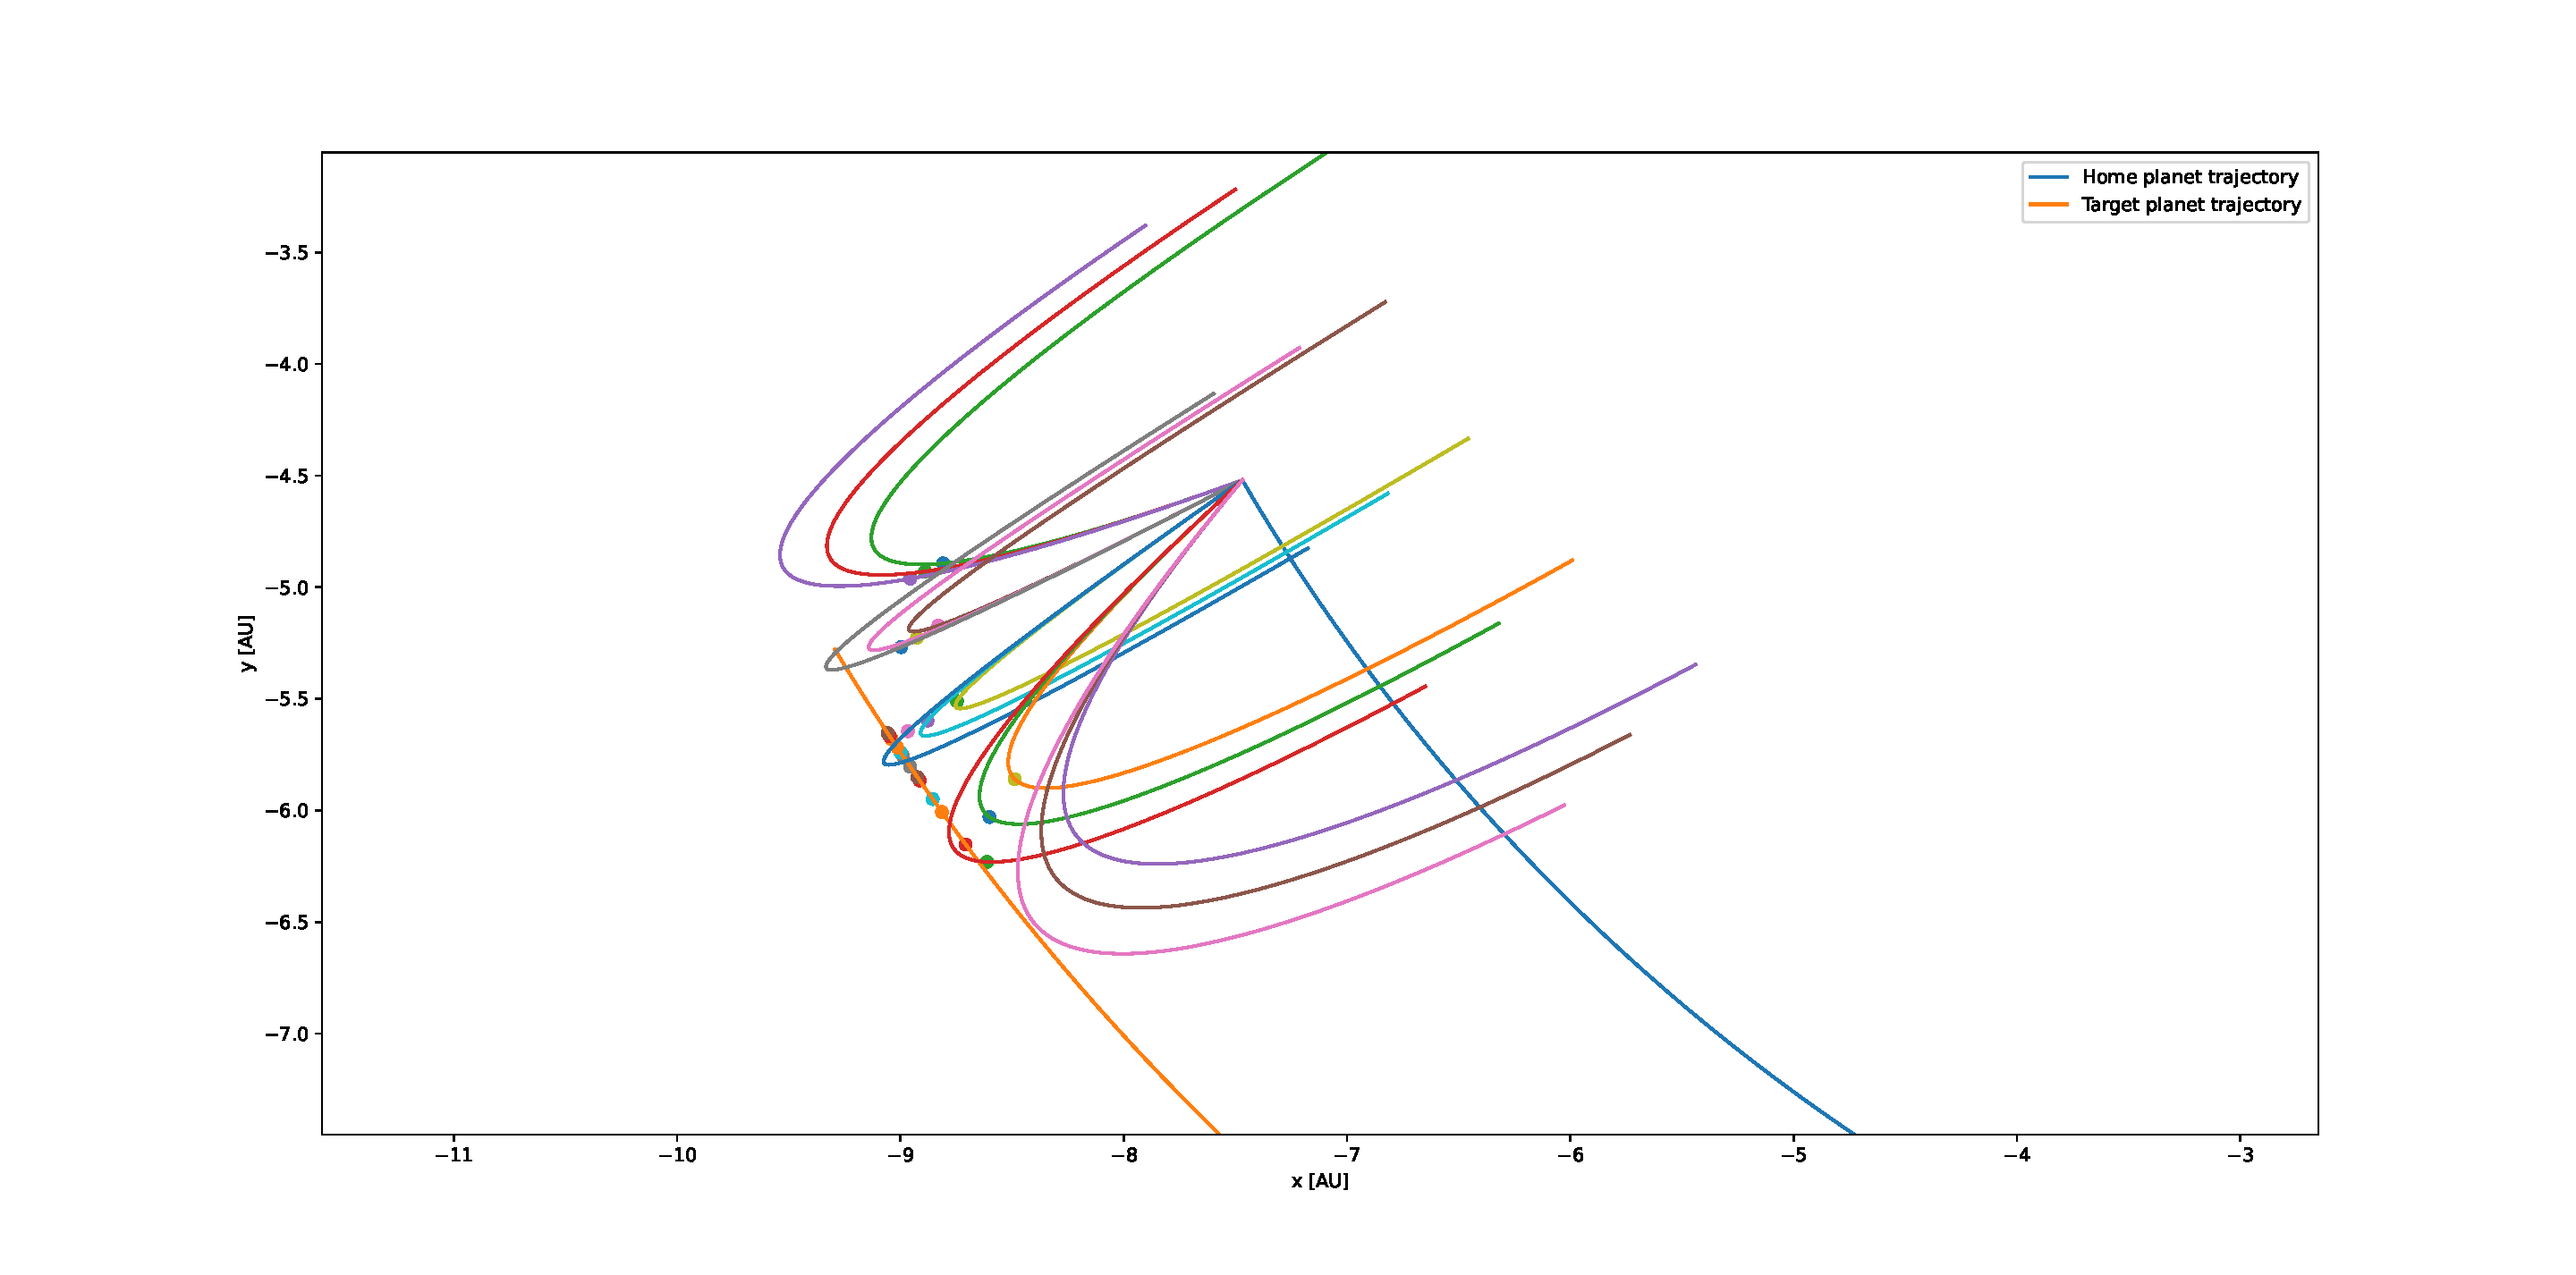
\includegraphics[scale = .185]{Figures/full_angle_scatter}
  \caption{Simulation of trajectory with relatively wide range of angles. The dots represent were the shuttle was the closest to the target planet }
  \label{fig: simulation scattered}
\end{figure}
In our case it seems our median angle was quite close.
Therefore, we only tighten up the span of angles by reducing the variance of angles.
We then get the following result in figure~\ref{fig: simulation tighter}.

\begin{figure}[h!]
  \centering
  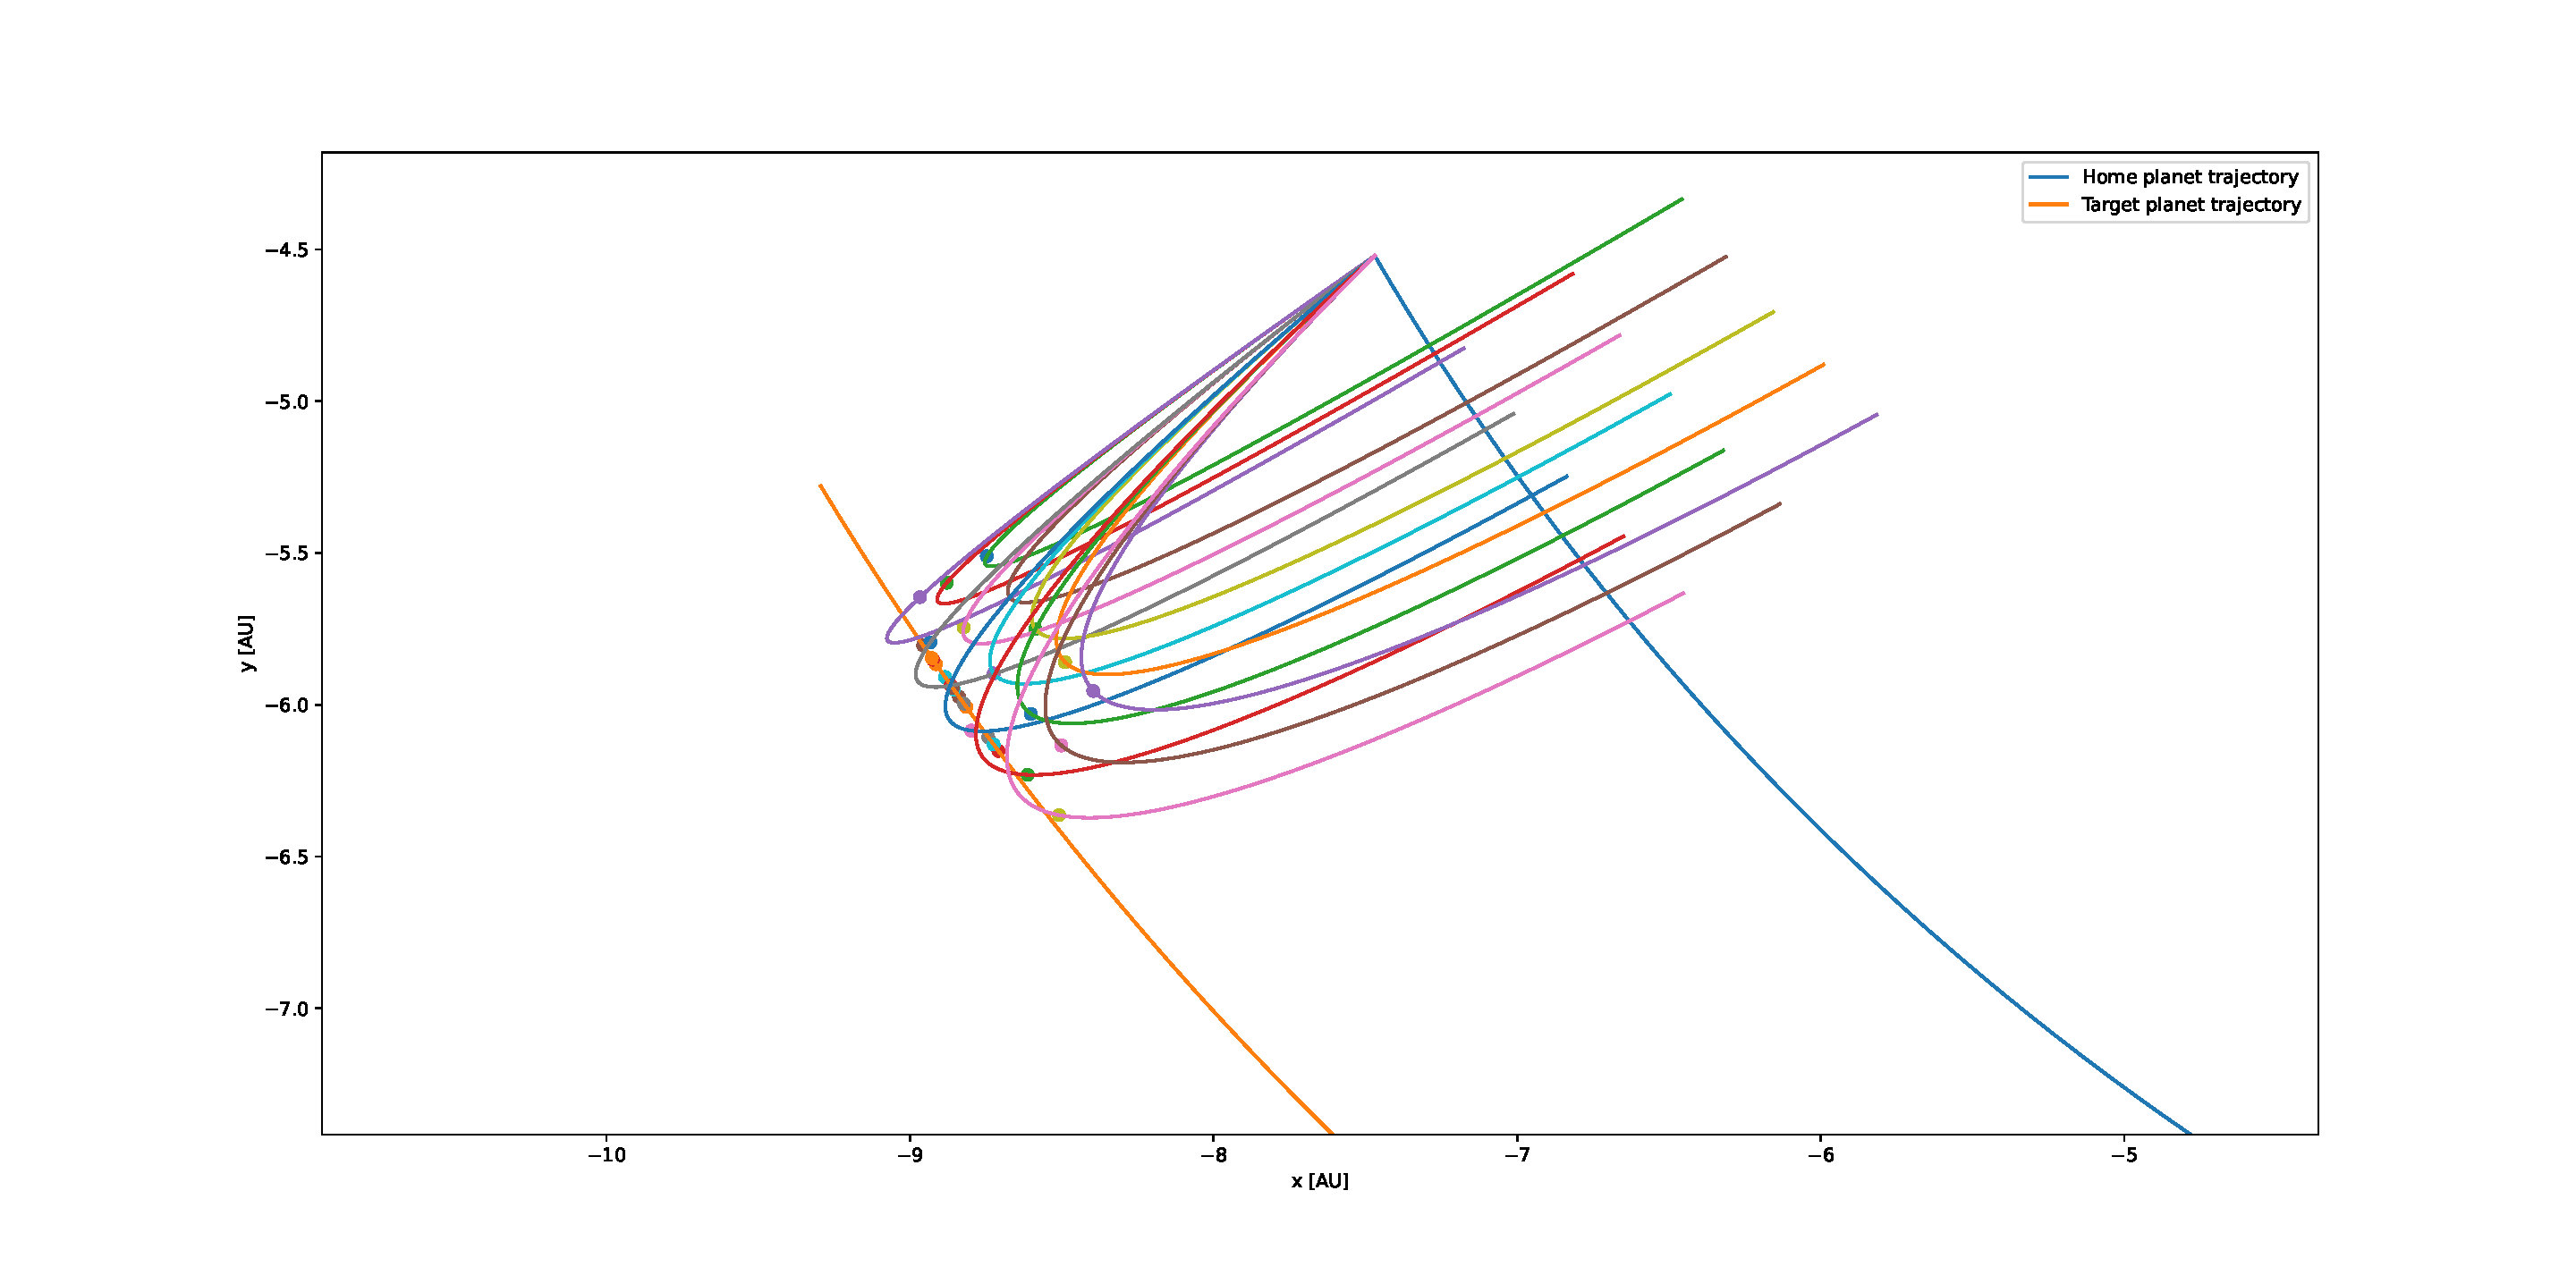
\includegraphics[scale = .185]{Figures/narrowing_down_angle}
  \caption{Simulation of trajectory after narrowing down the variance}
  \label{fig: simulation tighter}
\end{figure}

This is how we will find better and better values for our angle.
When it comes to the speed we will use the same technique.
As seen in the example from figure~\ref{fig: pre speed increase} our speed was too low in all three cases.

\begin{figure}[h!]
  \centering
  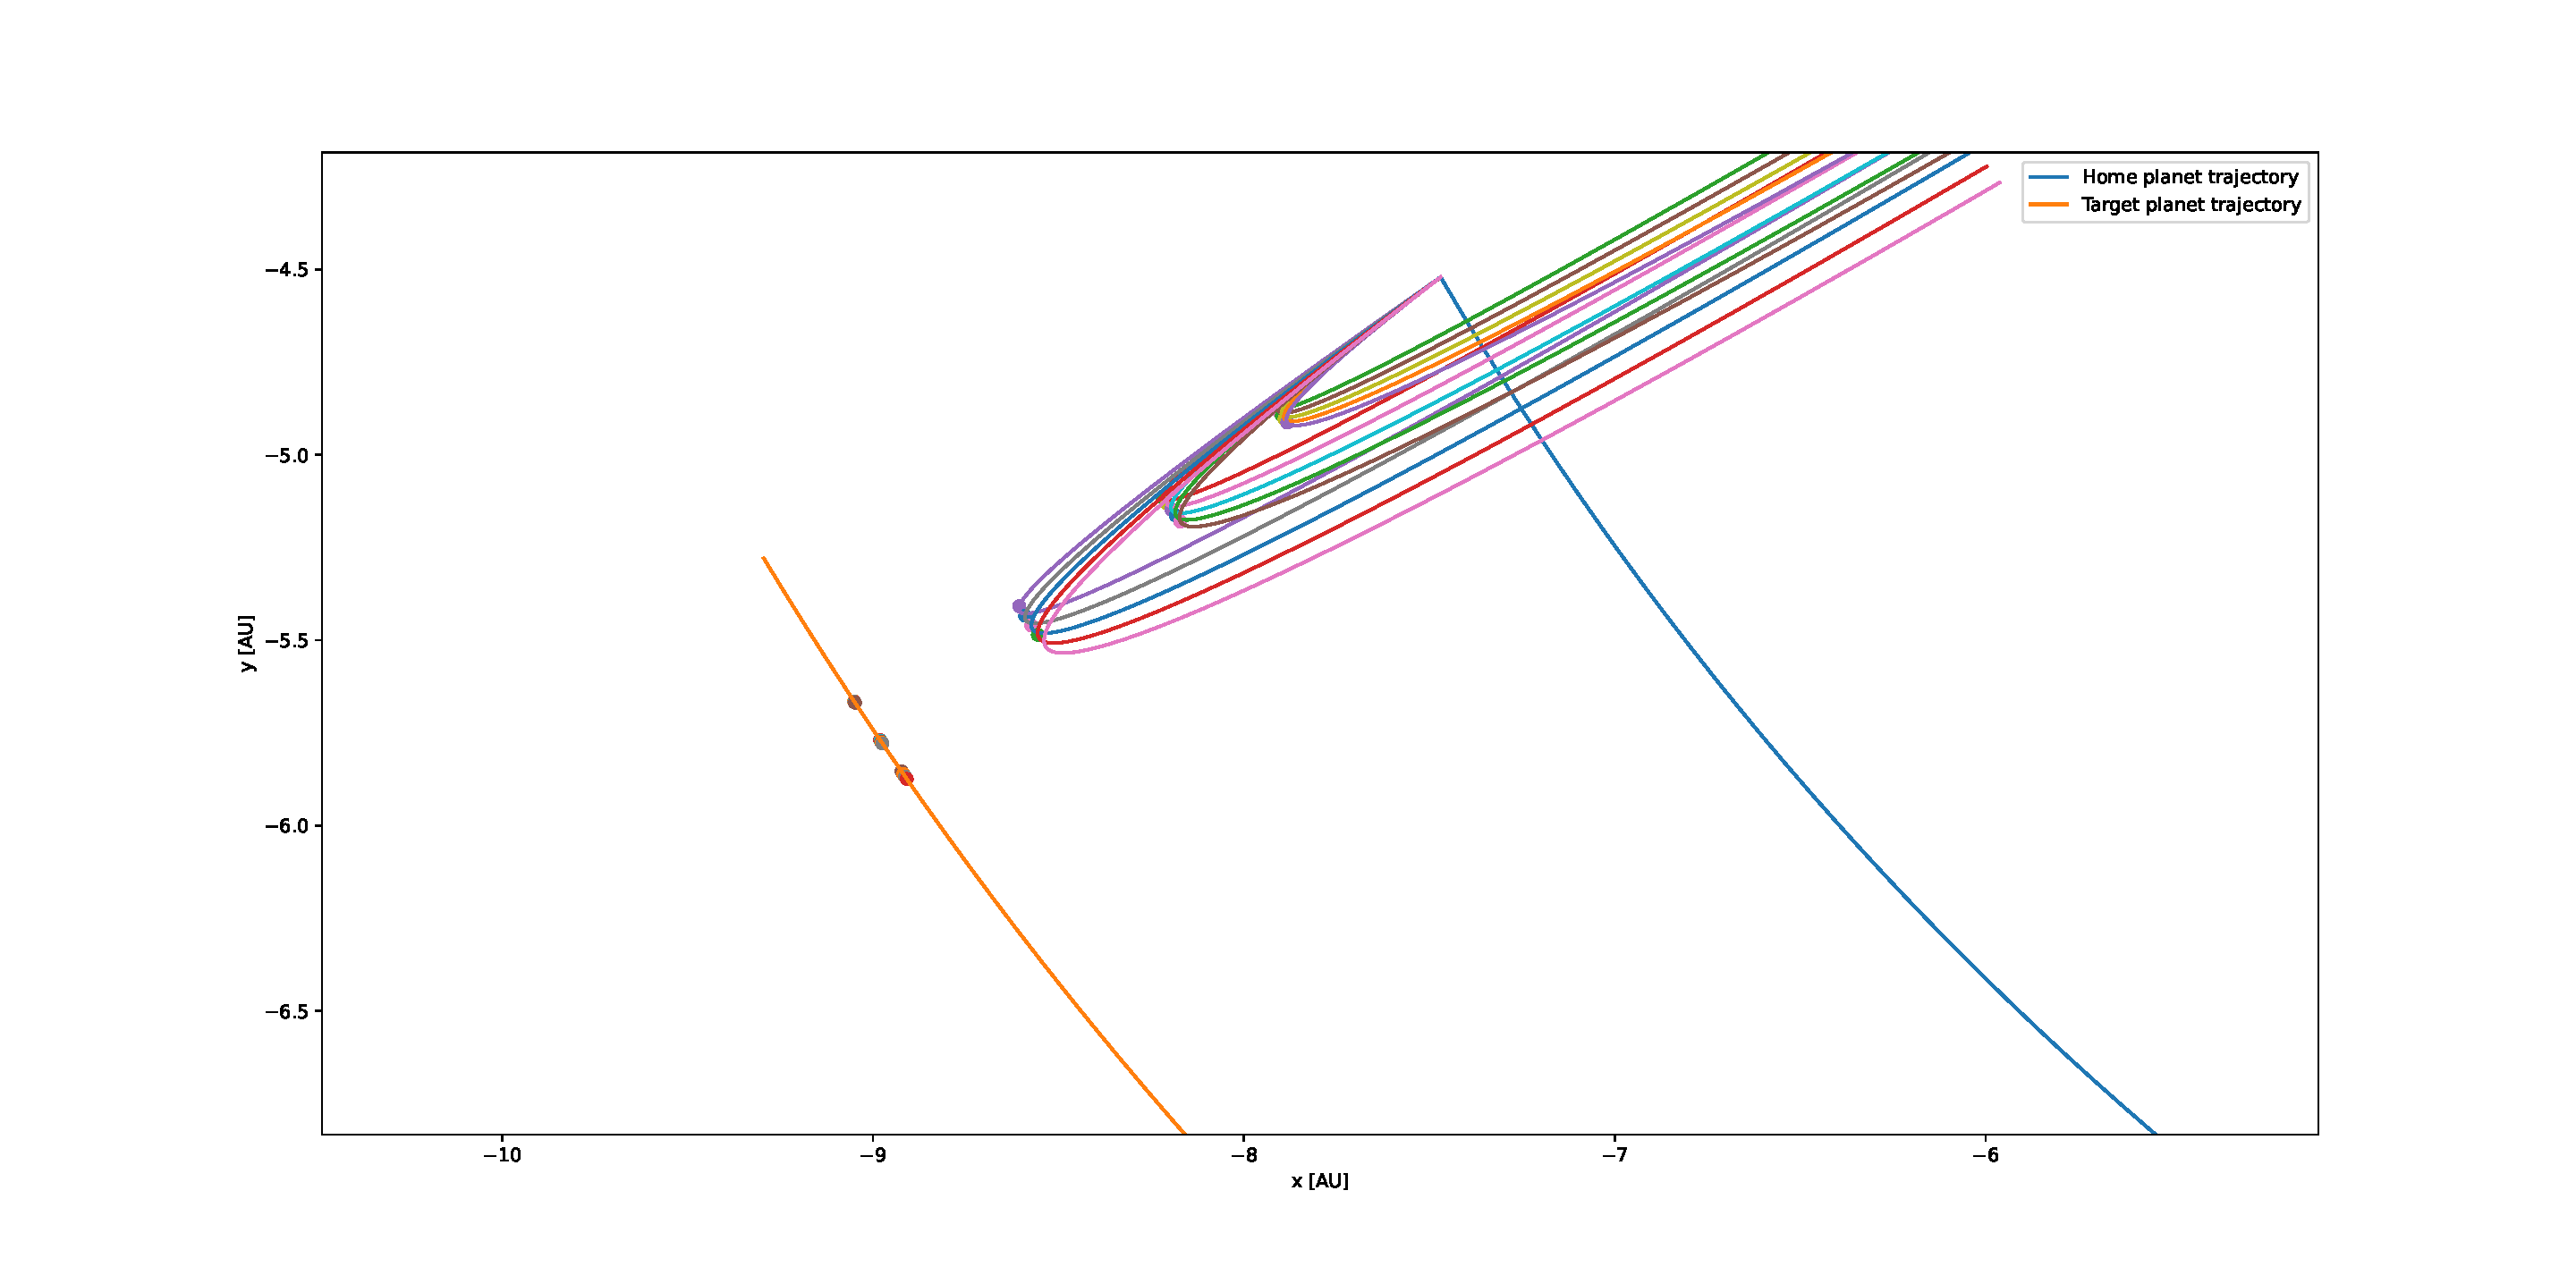
\includegraphics[scale = .185]{Figures/pre_speed_increase}
  \caption{Simulation of trajectory before speed increase}
  \label{fig: pre speed increase}
\end{figure}

Then it makes sense to increase it and check if we get closer.
When the speed was increased we got even closer to our target as seen in figure~\ref{fig: post speed increase}

\begin{figure}[h!]
  \centering
  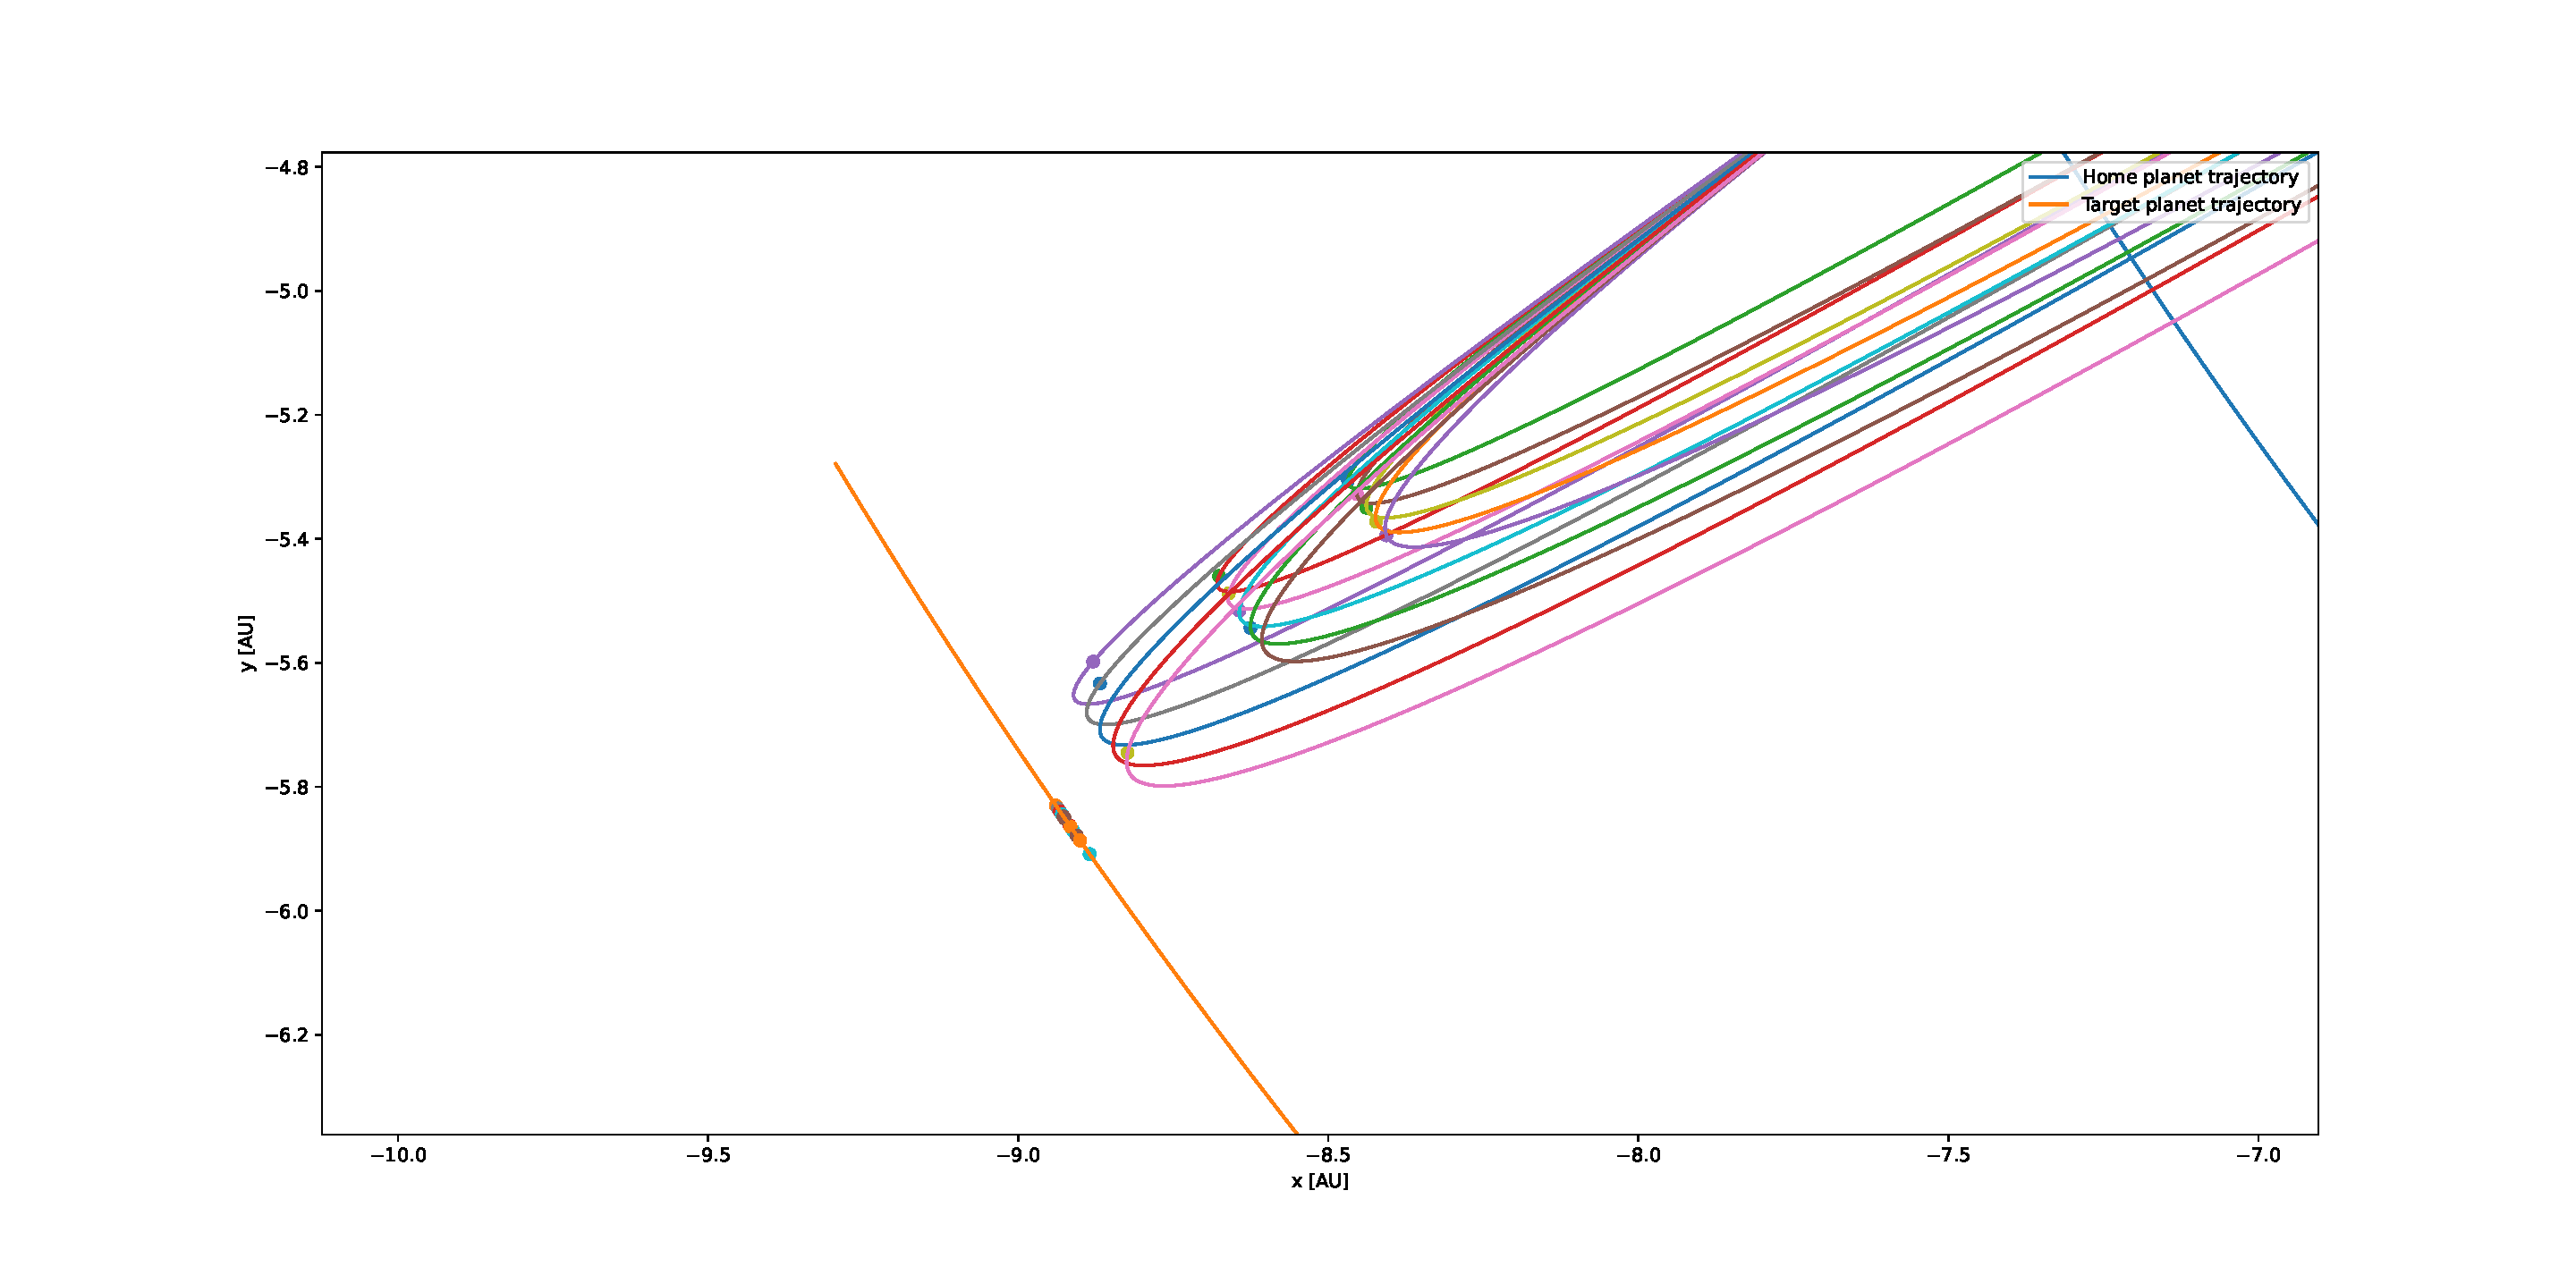
\includegraphics[scale = .185]{Figures/post_speed_increase}
  \caption{Simulation of trajectory after speed increase}
  \label{fig: post speed increase}
\end{figure}

These examples were to illustrate how we can refine our angles and velocity to get close enough to try and orbit the target planet.
For illustrative purposes we only used 5 different angles and three different speed, which gave us 15 different trajectories.
In reality, we will use hundreds of both to find the answer with as few adjustments as possible.
The simulation only yields the velocity the shuttle need in reference to our star in origin.
We subtract the velocity of our home planet from the calculated value to get the actual value our shuttle will need.


\subsection{Launching the Spacecraft}\label{subsec:launching-the-spacecraft}
    Having simulated the necessary parts of the launch, journey and conditions on our destination planet, we can now send the spacecraft on its journey.\\
    As stated in section~\ref{sec:introduction}, the time and direction of the launch will be based on our simulations.
    We will therefore launch the rocket at the point in time, which was deemed preferable in our simulations.\\

    After reaching space, the spacecraft will orient itself, and perform an initial boost to enter the simulated trajectory.
    To execute such a correctional boost, the onboard computer first calculates the required change in velocity.
    Thereafter, we use the onboard gyroscopic stabilizer to rotate the spacecraft.\\
    Since all forces acting on the spacecraft when it is coasting in space are conservative, the angular momentum must be conserved.
    The gyroscopic stabilizer uses three inertial wheels, which can be accelerated using electric motors to induce an angular momentum to the rocket due to the conservation of the total angular momentum.
    This means, we can rotate the rocket without using any fuel.\\
    After rotating the rocket, the main rocket engine will perform a short boost to change the velocity to the velocity required to enter the simulated trajectory.
    The exact duration of the boost, and therefore the change of velocity $\Delta \textbf{v}$ has been determined by the onboard computer.
    As we have measured the position $ \textbf{r}$ and velocity $\textbf{v}$ of the spacecraft when orienting ourselves after the launch, we can determine the required velocity $ \textbf{v}_{req}$ at the current position to enter a trajectory leading to the destination planet, using the method described in section~\ref{ssec: simulating trajectory} and~\ref{subsec:getting-close-enough}.
    The required change in velocity can then easily be found by subtracting.

    \begin{align}
        \Delta\textbf{v} = \textbf{v}_{req} - \textbf{v} \label{boost_calc_1}
    \end{align}

    However, this only gives us a vector.
    To find the direction and magnitude of the boost, we use some trigonometry.
    \begin{align} \label{boost_calc2}
        \Delta\textbf{v} = [\Delta v_x, \Delta v_y]\\
        |\textbf{v}| = \sqrt{{\Delta v_x}^2 + {\Delta v_y}^2}\\
        \theta = \arctan \left(\frac{\Delta v_y}{\Delta v_x}\right)
    \end{align}

    We then use the calculations from the first paper %~\parencite[][]{part1} TODO: Delete comment
    of this series of papers to calculate the amount of fuel used for a given $|\Delta\textbf{v}|$ in the process of the correction maneuver

    Since the duration of the calculations, rotation of the rocket and boost are insignificant compared to the duration of the journey to the destination planet, we will regard them as instantly.
    A representation of such a boost can be seen in figure~\ref{fig:boost_fig}.\\

    After the initial orientation and boost, the spacecraft will be departing on the planned trajectory to the destination planet.
    However, due to inaccuracies in the simulations, gravitational forces from small objects and solar winds, the actual trajectory of the spacecraft will deviate from the simulated trajectory.
    We will therefore orient the spacecraft at regular intervals and compare the position and velocity to the simulated trajectory.
    If the deviation is gets too large, we will initiate a correctional boost.
    This boost will be executed in exactly the same way as the initial boost after the launch of the spacecraft.\\

    The limit of the deviation, when we decide to initiate a boost needs to be chosen carefully as correctional boosts for smaller deviations require less fuel, but may need to happen more often.
    As we only have a limited amount of excess fuel after the launch, we need to be careful to be as efficient as possible when making corrections to our trajectory.\\
    This process of coasting on a trajectory, and correctional boosts will then be repeated until we arrive at the destination planet.

    The trajectory of the spacecraft will then end when we are within the required distance $l$ from the planet as calculated in section~\ref{subsec:getting-close-enough} and the velocity of the spacecraft relative to the planet only has a tangential component.
    In other words, if equation~\eqref{formula1} holds.
    \begin{align}
        \textbf{v}(t) \cdot \textbf{r}(t) = 0 \label{formula1}
    \end{align}
    At this point we have to perform another correctional boost in the opposite direction than our velocity to slow the spacecraft and enter into an orbit around the planet.
    The change of velocity $\Delta \textbf{v}$ depends on the velocity of the spacecraft before the boost, and the distance of the spacecraft to the center of the planet.\\
    The velocity $\textbf{v}_{tan}$ needed to be in a perfectly circular orbit can be calculated using the formula for the centripetal acceleration and the formula for gravitational acceleration.
    \begin{align*}
        a_c &= G \frac{M_{Planet}}{r^2}\\
        a_c &= \frac{\textbf{v}_{tan}^2}{r}\\
        v_{tan}^2 &= G \frac{M_{Planet}}{r}\\
        v_{tan} &= \sqrt{G \frac{M_{Planet}}{r}}
    \end{align*}
    Since both $ \textbf{v}$ and $\textbf{v}_{tan}$ are tangential velocities and therefore point in the same direction, we can now simply determine the required change in velocity $\Delta \textbf{v}$ by subtracting.
    \begin{align*}
        \Delta \textbf{v} = \textbf{v} - \textbf{v}_{tan}
    \end{align*}

    After this burn, the velocity of the spacecraft matches the velocity required to be in a perfectly circular orbit around the planet.
    The radius of the orbit has been measured and will remain constant.
    To determine the orbital period, we can use Kepler's third law of planetary motion~\eqref{Kepler3}.
    \begin{align}
        \frac{a^3}{T^2} = C \label{Kepler3}
    \end{align}


\subsection{The orbit around the destination planet}\label{subsec:the-orbit-around-the-destination-planet}
    Even though the spacecraft has performed an orbit injection maneuver which should lead to a perfectly circular orbit, the probability for unexpected things to happen is large.
    We therefore need to check what kind of orbit we ended up in after the injection maneuver.
    The first thing to do is to orient ourselves.
    This way, we can find out the position and velocity of the spacecraft relative to the planet.
    By determining our position and therefore the distance to the planet along the entire orbit and interpolating, we can find a function for the ellipse which makes up the orbit.
    Using this data, we can set up a two-body system as it is described in the second part of this series of papers%~\parencite[][]{part2}. TODO: Remove Comment
    This enables ut to describe the orbit as an ellipse with the planet in one of the focal points.
    The apoapsis and periapsis are given as the points on the orbit, which are respectively farthest and closest to the planet.
    The distances from these points to the planet are called the semi-major axis and semi-minor axis of the orbit
    By using formula~\eqref{formula2} we can determine the eccentricity $e$of the orbit.
    \begin{align}
        e = \sqrt{1-(b/a)^2} \label{formula2}
    \end{align}



    \section{Results} \label{sec: results}

    \begin{figure}[h]
      \centering
      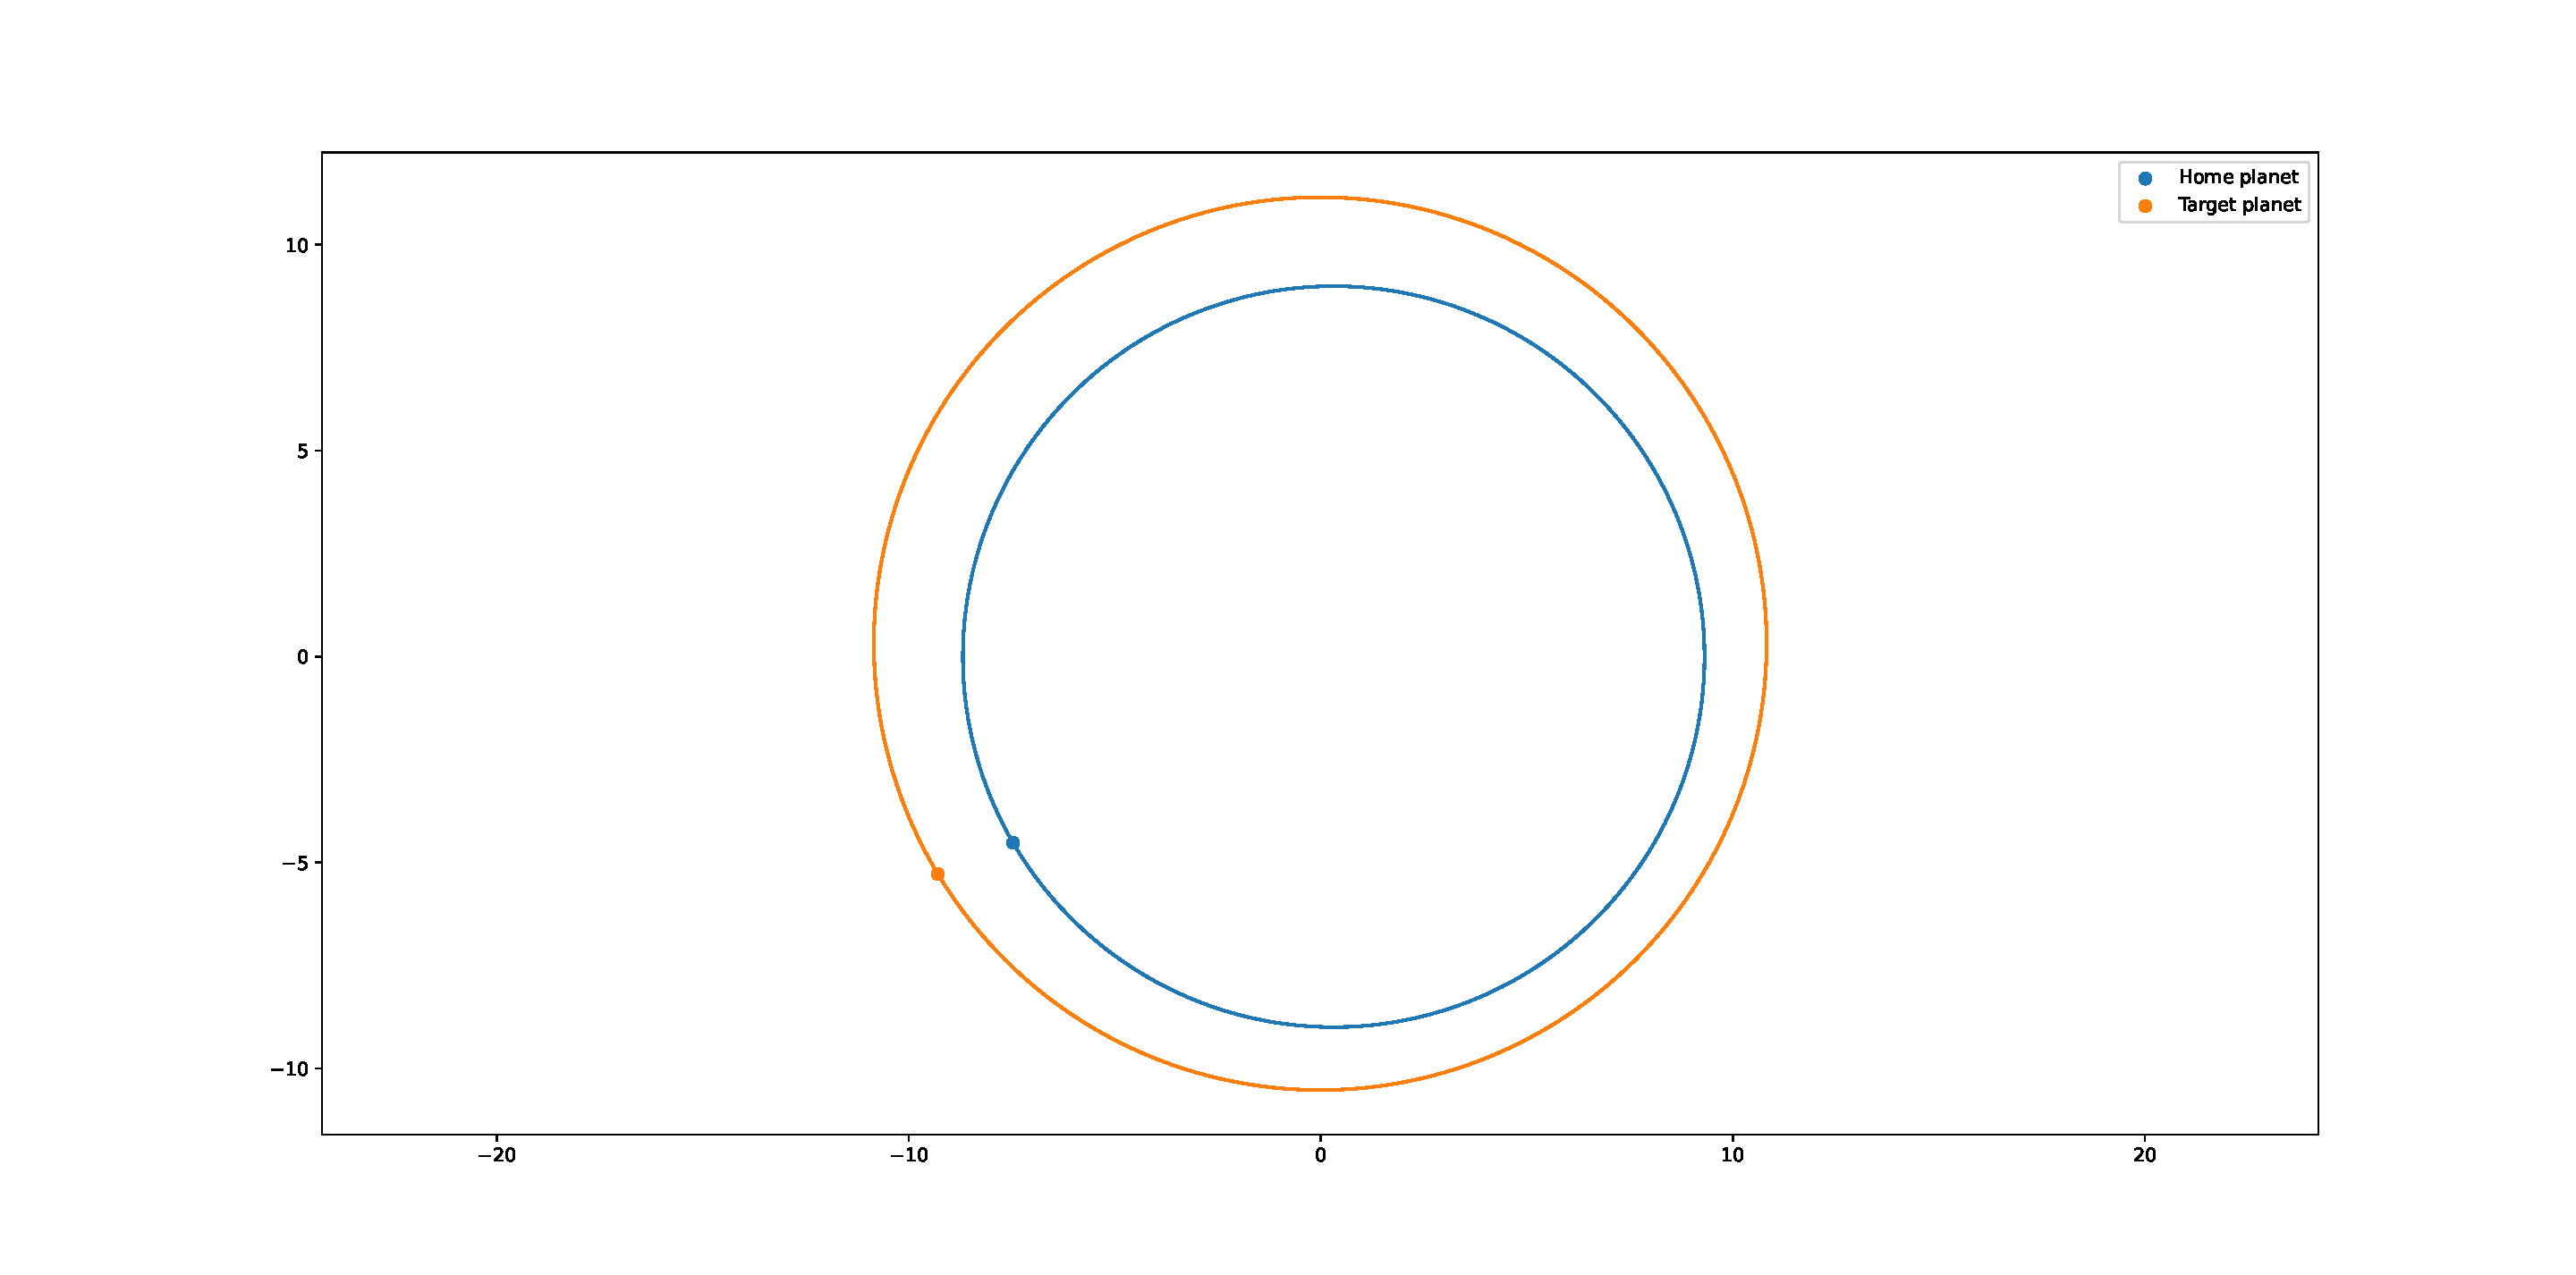
\includegraphics[scale = .2]{Figures/closest_orbit}
      \caption{Position where the target planet and our home planet were the closest}
      \label{fig: closest orbit}
    \end{figure}

    Our team of scientists have been very busy guiding the rocket to its final orbit around the destination planet, and have successfully completed the task.
    After launching the rocket, it successfully determined its position and velocity after reaching space.
    The launch happened at 08:33 on the 19th July of the year 238 in the timeframe of our solar system at an angle of $260.483^{\circ}$ and lasted 16 minutes and 36 seconds.
    This means the spacecraft reached space at 08:50.
    At this point in time, the spacecraft measured its position and velocity to be:
    \begin{align*}
        r_0 &= [-6.3033, -6.0995] \,\text{AU}\\
        v_0 &= [ 2.5919, -6.1838] \quad\text{AU/Year}
    \end{align*}

    However, this was not exactly the velocity $\textbf{v}_{req}$ we needed to enter the desired trajectory towards the destination planet.
    Therefore, a correction burn was performed.
    The required change of velocity $\Delta\textbf{v}$ was calculated using equations~\eqref{boost_calc_1} and~\eqref{boost_calc2}.
    After entering the simulated trajectory, the spacecraft coasted for 0.01 years, which equates to roughly 3 days and 15 hours and 36 minutes.\\
    Thereafter, the spacecraft oriented itself again to determine the deviation from the simulated trajectory.
    Multiple times, the deviation was large enough to require a correctional burn.
    These burns have been executed the same way as the first one after reaching space.\\
    After being closer than $9.601 \times 10^{-4}$ AU or $1.436 \times 10^5$ km, the gravitational forces from the destination planet started dominating.
    At this point, the spacecraft continuously monitored its movement relative to the planet and performed an orbit injection maneuver as it is described in section~\ref{subsec:launching-the-spacecraft}.
    This resulted in a circular orbit around the destination planet after 316 days and 8 hours of travel.\\
    The trajectory of the interplanetary travel can be seen in figure~\ref{fig:inter_trav}.
    \begin{figure}[h]
        %% H(Here), h(here approx), t(top of page), b(bottom of page)
        \centering
        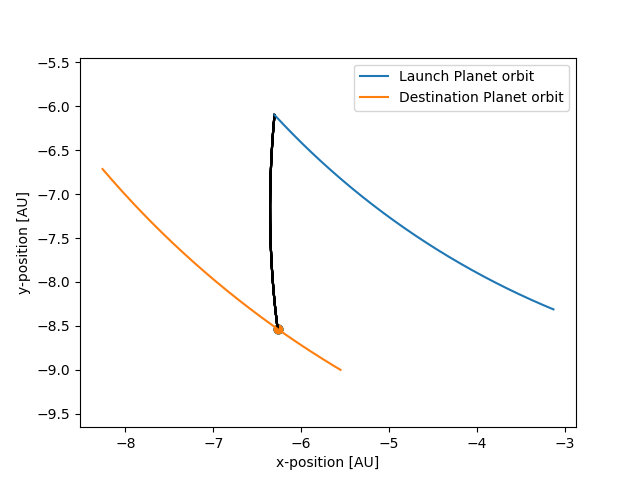
\includegraphics[scale=0.5]{Figures/inter_trav}
        \caption{The interplanetary travel of the spacecraft. The black line depicts the trajectory of the spacecraft.}\label{fig:inter_trav}
    \end{figure}

    The orbit was at an altitude of $7.5 \times 10^4$ km above the surface of the planet, which required a tangential velocity of $6.705$ AU/Year.
    Using Kepler's law the orbital period has been determined to be 7 hours 10 minutes and 35 seconds.

    \begin{figure}[h]
      \centering
      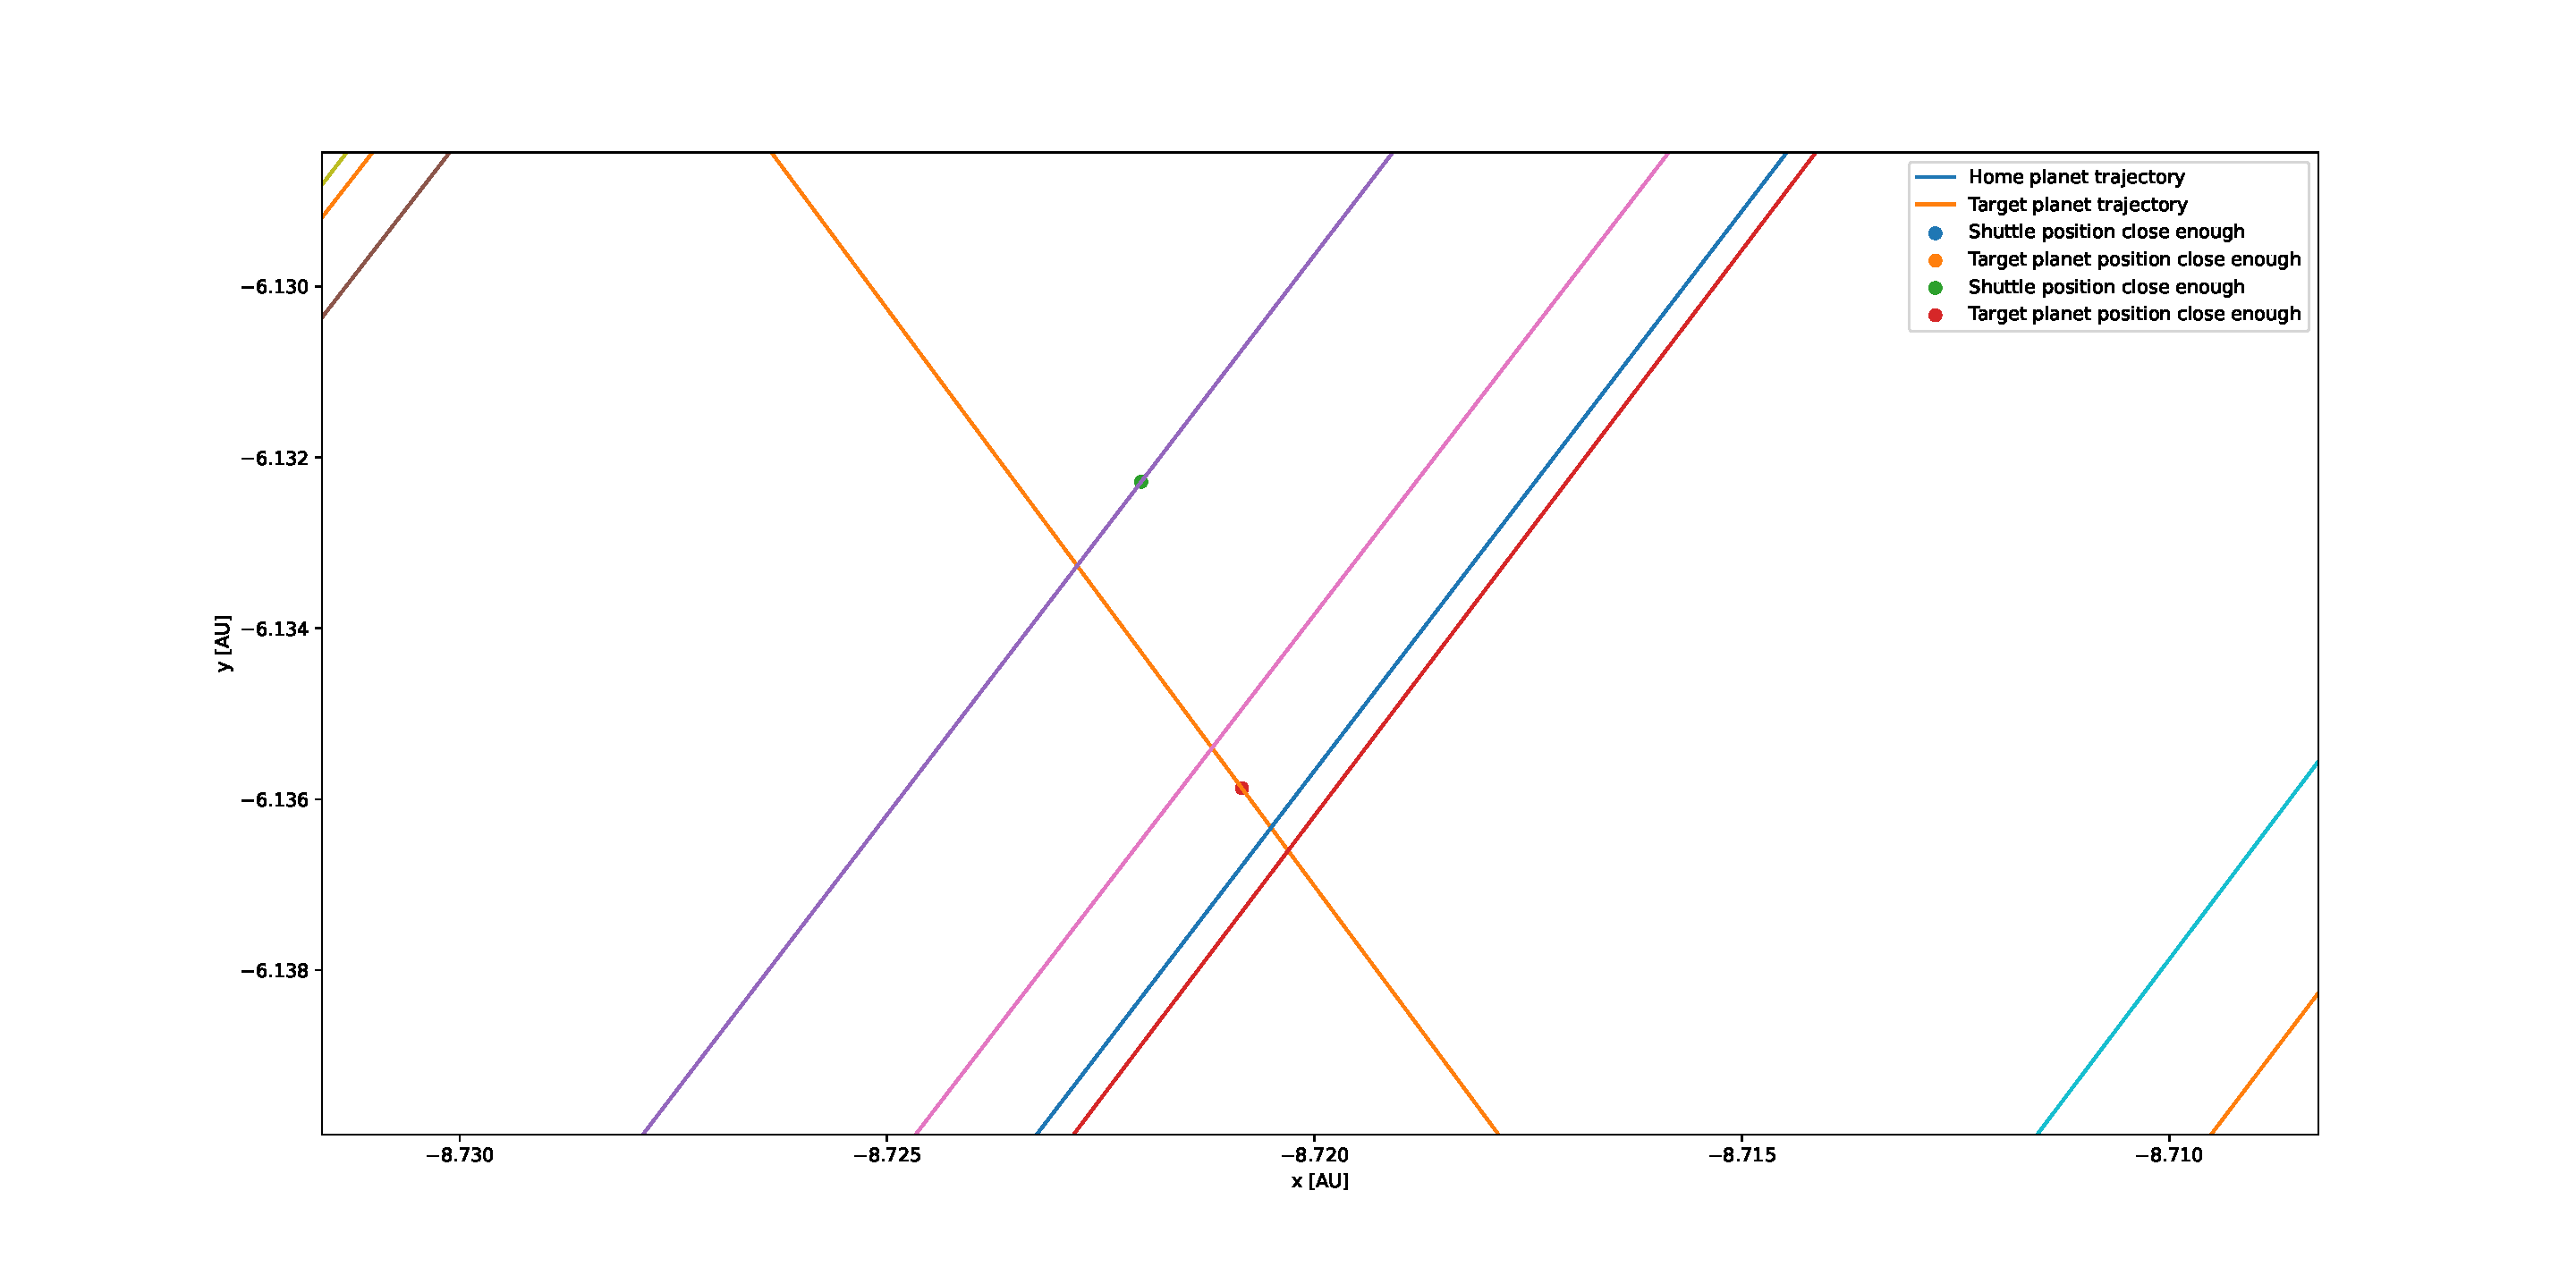
\includegraphics[scale = .19]{Figures/good_enough_distance}
      \caption{Position of shuttle and target planet at optimal distance for our simulated orbit. Lines depict trajectories at different angles}
      \label{fig: good enough distance}
    \end{figure}


\section{Discussion} \label{sec: discussion}
A lot of these calculations are based on the previous papers in this series of papers.
Hence, any uncertainties from these parts can impact calculations in this part.\\
This applies especially for the orbits of the planets in the solar system as these are numerically calculated.
As we do not have unlimited computing power, we had to trade some accuracy for shorter computing time.
This also applies for the numeric calculations of the simulated trajectory of this part.
However, due to advanced simulation algorithms, the errors induced could be reduced to a minimum and therefore, the impact on the end result should not lead to very large deviations.\\
Furthermore, a lot of our calculations include gravitational forces, which are dependent on the mass of objects.
It is relatively simple to determine the mass of our spacecraft, but since we are not able to determine the mass of the planets and the star in our solar system using scales, these might not be entirely exact.
Even though our scientists have found very good methods for these applications, there will always be some uncertainties.

\subsection{Forces during launch and trajectory}\label{subsec:the-launch}
    Other things impacting the results of our simulations and the journey of the spacecraft are forces, which we did not account for.
    During the launch this includes the aerodynamic drag, which we neglected but actually exerts quite a significant force at higher velocities.
    We might therefore not reach the height or velocity we simulated and wanted to reach.\\
    This is quite dangerous as the rocket could either fall back to earth at a different place, which might be populated.
    The rocket could also end up in something called a gravitational slingshot, which transfers some of the planet's momentum to the spacecraft and launches it into another, unspecified trajectory.\\

    After the launch from our home planet, and entering space, there will be further forces which are difficult to foresee and therefore account for.
    We are of course aware of the larger objects in our solar system like the planets and star, which exert most of the gravitational forces on the spacecraft.
    However, there are thousands of small objects such as meteoroids in space, which exert small gravitational forces.
    These forces are relatively small, but can still have an effect on the trajectory of the spacecraft when close enough.\\
    Furthermore, the star continuously expels clouds of ions into the solar system due to the violent fusion processes in its core.
    These are called solar winds and exert a small, but continuous force on the spacecraft, which can further impact its trajectory.
    These forces are unaccounted for in our simulations, which could lead to significant deviations.

\subsection{The Spacecraft}\label{subsec:the-spacecraft}
    Another source of error can be the spacecraft itself.
    Even though we are using cutting edge technology, there will always be a small chance of an error, which could lead to uncertainties in measurements such as when orienting ourselves and measuring our velocity.
    Furthermore, the behaviour of the rocket engine in space can differ from what we expect and therefore induce combustion instabilities, which can make it difficult to perform a precise correctional burn.\\
    An assumption which might impact our results as well, is the duration of the correctional boost.
    We assumed these to be instant, whereas they do have some duration in reality.
    This could mean that the spacecraft does not enter the exact calculated trajectory, which we wanted after the boost.
    However, as we are checking the deviance from the simulated trajectory at regular intervals, this error would most likely be corrected during the next boost, resulting in the spacecraft reaching its destination nevertheless.

\subsection{Entering Orbit}\label{subsec:entering-orbit}
    Looking at the orbital injection maneuver, we also see some possible error sources.
    The burn which is meant to slow down the spacecraft has a duration, as all other correctional burns did.
    This means, we would have to start this burn a little earlier than we did in our simulations.
    Not doing so, or failing to do it at the perfect point in time would lead to entering into an elliptical orbit.\\
    We entered a perfectly circular, and therefore a stable orbit, but the chances for achieving this are extremely low.
    This result should therefore be seen very critically.
    If we entered an elliptical orbit instead, we would have to perform correctional boosts to enter a more stable orbit.\\
    Just like when travelling in space, we will also be influenced by small objects while executing the orbital injection maneuver and while being in orbit around the planet.
    This makes if even more difficult to achieve a perfectly circular orbit.\\

    As we are still rather far up in orbit, the atmosphere is extremely thin, but staying in the orbit for prolonged periods of time will still require us to perform correctional boosts.
    The perfectly circular orbit will therefore most likely not stay circular forever if the spacecraft simply coasts.
    There will be minimal amounts of friction which can vary and brake the spacecraft at different times and alter the orbit.
    However, after orbiting around the planet multiple times and measuring the orbit again, we could confirm that the orbit we entered was stable.



\section{Conclusion} \label{sec: conclusion}
    After simulating all parts of the journey of the spacecraft to the destination planet, we were finally able to launch it.
    Using the simulations, necessary parameters such as thrust, launch angle and favorable time of launch for a successful launch could be determined.
    The launch happened at 08:33 on the 19th July of the year 238, and went well
    This lead to a successful orientation of the spacecraft after reaching space and entering into the predetermined trajectory towards the destination planet, which was simulated using the orbital mechanics and the leapfrog algorithm.
    During the travel from the launch planet to the destination planet, multiple trajectory corrections were necessary to keep the spacecraft on the predetermined trajectory.
    After 316 days and 8 hours of travel, the spacecraft finally reached its destination and initialised an orbit injection maneuver.
    The injection maneuver slowed the spacecraft sufficiently to enter into orbit around planet 1.
    This was a very critical maneuver, since small deviations could lead to the spacecraft entering an elliptical, and therefore unstable orbit.
    Thanks to precise boosts, we were able to enter a circular, and therefore stable orbit.
    To confirm the shape and stability of the orbit, the orbit was calculated again based on the position and velocity of the spacecraft after multiple orbits.
    We were therefore able to confirm successful travel to planet 1 and entry into a stable orbit at an orbital height of 75'000 km above the surface.


\newpage
% \printbibliography TODO: Remove Comment
\end{document}